\documentclass{ximera}
\input{../preamble}
\addPrintStyle{..}

% 

\begin{document}
	\author{Zomercursus KU Leuven}
	\xmtitle{Intro: nieuwe getallen voor meetkunde}{}
	
	\label{xim:inleiding_meetkundig}

	% Inspiratie: zie filmpje Burgerlijk Ingenieurs (K. Paes)
	% Inspiratie: zie https://www.projectx2002.org/Wiskunde/Vijfdes/Cursus%20Complexe%20Getallen.pdf   (S. Mettepeningen)

	Het woord \textit{getallen} is afgeleid van \textit{tellen}, zoals bij één appel, twee appels, drie appels,\ldots. 
	Je kan met getallen echter ook \textit{meten} in plaats van tellen, zoals bij één meter of twee meter, en dan kunnen ook kommagetallen zoals 1,5 meter of 3,14 meter voorkomen.
	En als je temperaturen wil meten heb je ook negatieve getallen als -10 of -272 nodig.
	% Je kan getallen ook gebruiken om te vermenigvuldigen, en dus te berekenen dat een kamer van 3 meter bij 5 meter een oppervlakte heeft van 15 \si{m^2}.
    %Getallen worden echter ook dikwijls gebruikt om iets te \textit{herschalen}, of daarmee gerelateerd, om \textit{verhoudingen} weer te geven.

	\begin{image}[\textwidth]
		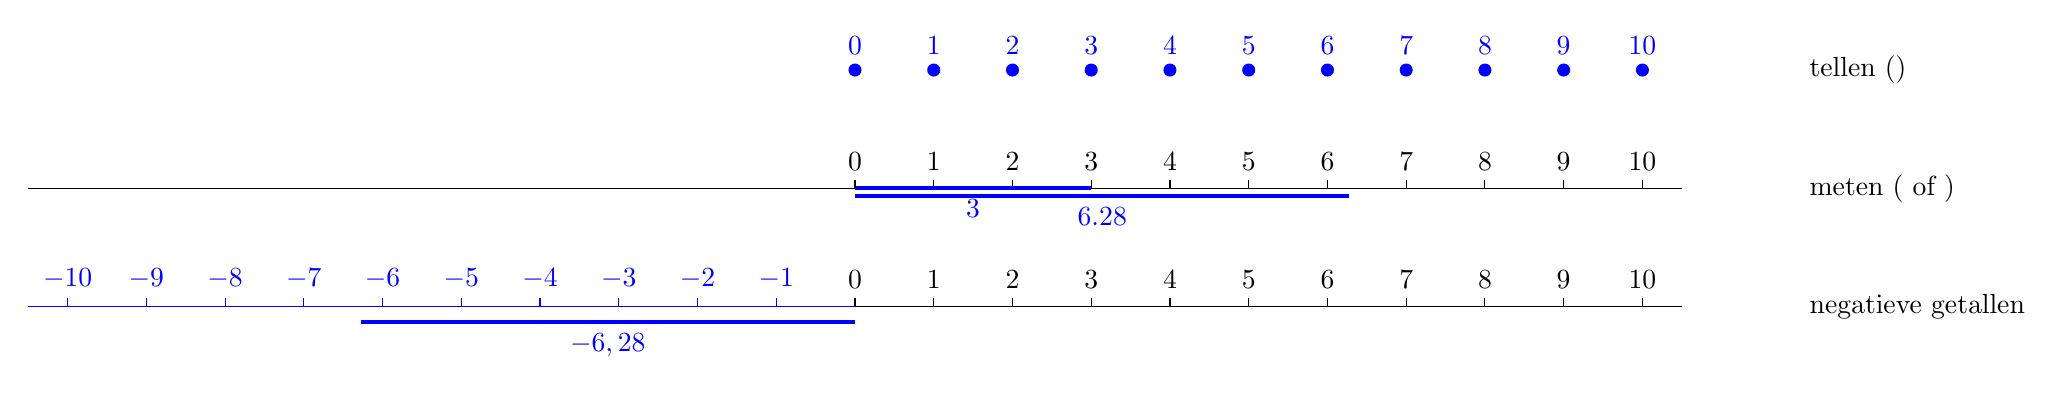
\begin{tikzpicture}
	
			\draw (12,0) node [right] {\blue{tellen} ($\N$)};
			\foreach \x in {0,1,...,10} {
				\draw[blue] (\x,0) node[fill,circle,radius=1pt,scale=0.5] {} node[above,yshift=2pt,] {$\x$};
			}
	
			\begin{scope}[yshift=-1.5cm]
			\draw (12,0) node [right] {\blue{meten} ($\Q$ of $\R$)};
			\draw (-10.5,0) -- (10.5,0);
			\draw[blue, ultra thick] (0,0) --  node[below] {$3$} (3,0);
			\draw[blue, ultra thick] (0,-0.1) --  node[below] {$6.28$} (6.28,-0.1);
			\foreach \x in {0,1,...,10} {
				\draw (\x,0) -- (\x,0.1) node[above] {$\x$};
			}
			\end{scope}

			\begin{scope}[yshift=-3cm]
			\draw (12,0) node [right] {\blue{negatieve getallen}};
			\draw (-10.5,0) -- (10.5,0);
			\draw[blue] (-10.5,0) -- (0,0);
			\draw[blue, ultra thick,yshift=-0.2cm] (0,0) --  node[below] {$-6,28$} (-6.28,0);
			%\draw[blue, ultra thick] (0,-0.1) --  node[below] {$6.28$} (6.28,-0.1);
			\foreach \x in {-10,-9,...,-1} {
				\draw[blue] (\x,0) -- (\x,0.1) node[above] {$\x$};
			}
			\foreach \x in {0,1,...,10} {
				\draw (\x,0) -- (\x,0.1) node[above] {$\x$};
			}
			\end{scope}

		\end{tikzpicture}			
	\end{image}


			

	In dit hoofdstuk maak je kennis met een nieuw soort getallen.
	En met deze nieuwe getallen kan je nieuwe dingen doen, die onmogelijk zijn met de getallen die je al kent.

	%%%  Mmm, taarten verdelen werkt niet met vierkantswortels; beter iets met vergroten: zie infra
	%%%
	% Iedereen weet dat het dikwijls nuttig is om dingen in stukken te verdelen. 
	% Als je een taart verdeelt in vier gelijke stukken, dan is elke stuk taart één vierde van de hele taart, en de som van de vier vierden is terug de hele taart.
	% In een formule wordt dat 
	% $$
	% 1 = \frac14 + \frac14 +\frac14 +\frac14.
	% $$
	% Als je de taart effectief in vier stukken wil snijden, gebeurt dat meestal door ze twee keer in de helft door te snijden:
	% $$
	% \frac{1}{2}\times 1 = \frac12 + \frac12
	% $$


    We focussen op het gebruik van getallen om te herschalen. Het getal $3$ kan dienen om alles met een factor drie te vergroten. Door dat twee keer na elkaar te doen, wordt er natuurlijk vergroot met een factor $3\times3=9$.

	\begin{image}[\textwidth]
		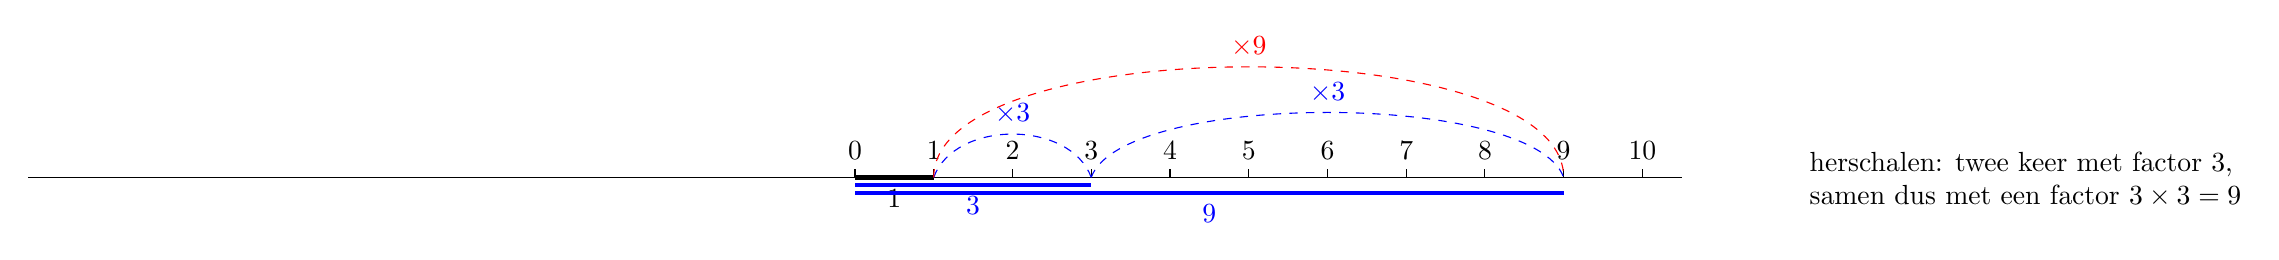
\begin{tikzpicture}
	
		\begin{scope}[yshift=-4cm]
		\draw (12,-0.5) node [above right, align=left] {\blue{herschalen}: twee keer met factor $\blue{3}$,\\samen dus met een factor $3\times3=\red{9}$};
		\draw (-10.5,0) -- (10.5,0);
		\draw[black, ultra thick] (0,0) --  node[below=0.2] {$1$} (1,0);
		\draw[blue, ultra thick] (0,-0.1) --  node[below=0.1] {$3$} (3,-0.1);
		\draw[blue, ultra thick] (0,-0.2) --  node[below] {$9$} (9,-0.2);
		\foreach \x in {0,1,...,10} {
			\draw (\x,0) -- (\x,0.1) node[above] {$\x$};
		}
		\draw[blue, dashed] (1,0) edge[in=110,out=70]  node[above] {$\times 3$} (3,0);
		% \draw[red, dashed] (3.14,0) edge[in=110,out=70]  node[above] {$\times 2$} (6.28,0);
		\draw[blue, dashed] (3,0) edge[in=110,out=70,looseness=0.5]  node[above] {$\times 3$} (9,0);
		\draw[red, dashed] (1,0) edge[in=90,out=90,looseness=0.6]  node[above] {$\times 9$} (9,0);

		\end{scope}
	\end{tikzpicture}			
\end{image}


	%De omgekeerde uitdaging is meestal groter. Inderdaad, als we in twee keer met in totaal een factor $9$ willen vergroten, volstaat het twee keer met $3$ te vergroten. 
    Maar stel dat we \textit{in twee stappen} met in totaal een factor $3$ willen vergroten? Dan hebben we een getal $x$ nodig zodat $x \times x = 3$, en dergelijk getal is $\sqrt{3}$, de vierkantswortel van $3$.


	\begin{image}[\textwidth]
		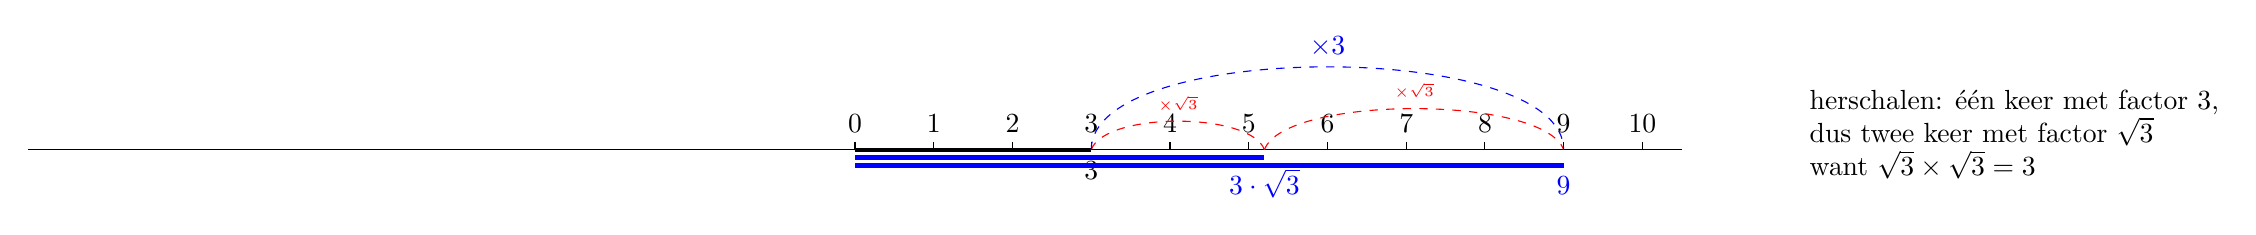
\begin{tikzpicture}

		\begin{scope}[yshift=-6.5cm]
		\draw (12,-0.5) node [above right, align=left] {\blue{herschalen}: één keer met factor $\blue{3}$,\\dus twee keer met factor $\red{\sqrt{3}}$\\ want $\sqrt{3}\times\sqrt{3}=3$};
		\draw (-10.5,0) -- (10.5,0);
		\draw[ultra thick] (0,0)    --  (3,0)    node[below=0.2] {$3$} ;
		\draw[blue, ultra thick] (0,-0.1) --  (5.2,-0.1) node[below] {$3\cdot\sqrt{3}$} ;
		\draw[blue, ultra thick] (0,-0.2) --  (9,-0.2) node[below] {$9$} ;
		\foreach \x in {0,1,...,10} {
			\draw (\x,0) -- (\x,0.1) node[above] {$\x$};
		}
		%\draw[red, dashed] (1,0) edge[in=110,out=70]  node[above] {$\scriptscriptstyle\times \sqrt{3}$} (1.73,0);  % sqrt(3)=1.73...
		%\draw[red, dashed] (1.73,0) edge[in=110,out=70]  node[above] {$\scriptscriptstyle\times \sqrt{3}$} (3,0);
		%\draw[red, dashed] (1,0) edge[in=110,out=70,looseness=1.5]  node[above] {$\scriptstyle\times \sqrt{3}\times\sqrt{3} = \times 3$} (3,0);
		% \draw[red, dashed] (3.14,0) edge[in=110,out=70]  node[above] {$\times 2$} (6.28,0);
		\draw[red, dashed] (3,0)   edge[in=110,out=70,looseness=0.6]  node[above] {$\scriptscriptstyle\times \sqrt{3}$} (5.2,0);
		\draw[red, dashed] (5.2,0) edge[in=110,out=70,looseness=0.5]  node[above] {$\scriptscriptstyle\times \sqrt{3}$} (9,0);
		\draw[blue, dashed] (3,0)  edge[in=90 ,out=90,looseness=0.6]  node[above] {$\times 3$} (9,0);
		\end{scope}
	\end{tikzpicture}			
\end{image}

%    Door te vermenigvuldigen met $-1$ spiegelen we de getallenrechte: alle positieve getallen worden negatief en omgekeerd. 
Vermenigvuldigen met -1 is spiegelen rond de oorsprong, als volgt:


\begin{image}[\textwidth]
	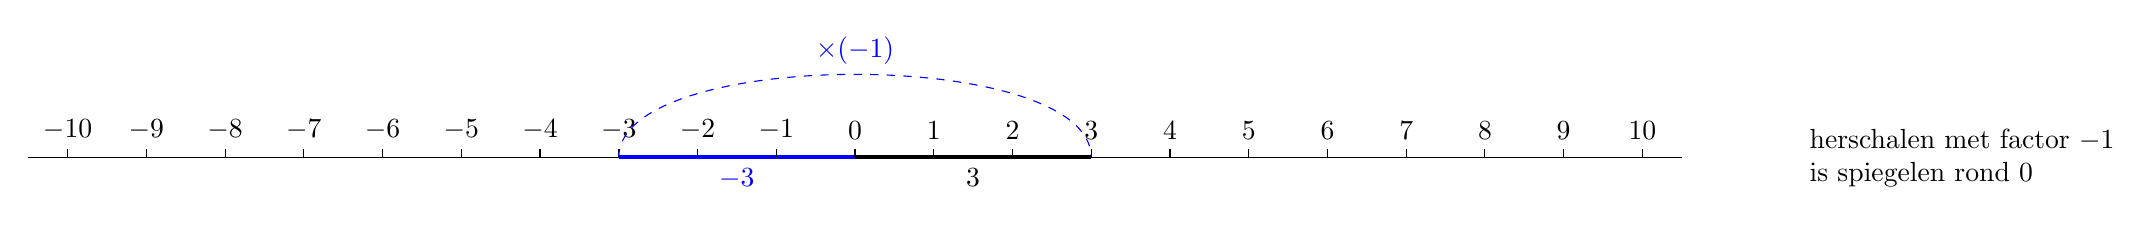
\begin{tikzpicture}

	\draw (12,-0.5) node [above right,align=left] {\blue{herschalen} met factor $-1$\\ is spiegelen rond $0$};
	\draw (-10.5,0) -- (10.5,0);
	\draw[ultra thick] (0,0) --  node[below] {$3$} (3,0);
	\draw[blue, ultra thick] (-3,0) --  node[below] {$-3$} (0,0);
	\foreach \x in {-10,-9,...,10} {
		\draw (\x,0) -- (\x,0.1) node[above] {$\x$};
	}
	%\draw[blue, dashed] (-1,0) edge[in=110,out=70] (1,0);
	% \draw[red, dashed] (3.14,0) edge[in=110,out=70]  node[above] {$\times 2$} (6.28,0);
	\draw[blue, dashed] (-3,0) edge[in=90,out=90,looseness=0.6]  node[above] {$\times (-1)$} (3,0);

\end{tikzpicture}
\end{image}
	
	Men kan zich afvragen of op één of andere manier ook het spiegelen van de getallenrechte kan worden opgesplitst in het herhalen van twee keer dezelfde operatie.

	\begin{image}[\textwidth]
		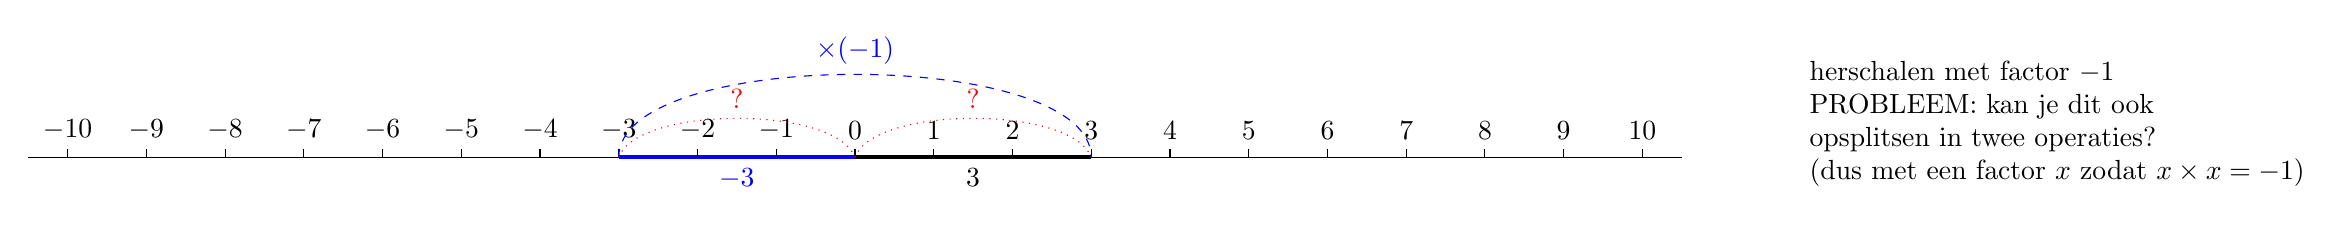
\begin{tikzpicture}

		\begin{scope}[yshift=-9cm]
		\draw (12,-0.5) node [above right,align=left] {\blue{herschalen} met factor $-1$\\ \red{PROBLEEM}: kan je dit ook \\\red{opsplitsen in twee operaties?}\\ (dus met een factor $x$ zodat $x\times x = -1$)};
		\draw (-10.5,0) -- (10.5,0);
		\draw[ultra thick] (0,0) --  node[below] {$3$} (3,0);
		\draw[blue, ultra thick] (-3,0) --  node[below] {$-3$} (0,0);
		\foreach \x in {-10,-9,...,10} {
			\draw (\x,0) -- (\x,0.1) node[above] {$\x$};
		}
		%\draw[blue, dashed] (-1,0) edge[in=110,out=70] (1,0);
		% \draw[red, dashed] (3.14,0) edge[in=110,out=70]  node[above] {$\times 2$} (6.28,0);
		\draw[blue, dashed] (-3,0) edge[in=90,out=90,looseness=0.6]  node[above] {$\times (-1)$} (3,0);
		\draw[red, dotted] (-3,0) edge[in=110,out=70,looseness=0.6]  node[above] {?} (0,0);
		\draw[red, dotted] (0,0) edge[in=110,out=70,looseness=0.6]  node[above] {?} (3,0);
		\end{scope}

	\end{tikzpicture}
\end{image}


    \begin{denkvraag*}{}
        Denk je dat het mogelijk is om een operatie op de getallenas te vinden zodat deze operatie twee keer na elkaar uitvoeren de getallenas spiegelt rond te oorsprong?
    \end{denkvraag*}


	
% Als je wil in twee gelijkwaardige stappen wil herschalen met een factor $4$, kan dat makkelijk door twee keer mat een factor $2$ te herschalen. 
% Op dezelfde manier kan je door twee keer met een factor $5$ te herschalen, een herschaling met factor $25$ in twee keer doen.
% Hoe kan je echter een herschaling  met een factor $3$ in twee even grote stappen doen? Wel, je moet dan twee keer herschalen met een factor $\sqrt{3}$. Inderdaad, door twee keer met een factor $\sqrt{3}$ te vermenigvuldigen, heb je in totaal met een factor $\sqrt{3}\times\sqrt{3}=\sqrt{3\times3} =  \sqrt{9}=3$ vermenugvuldigd.

% De vraag van één miljoen die complexe getallen voor ons oplossen is: hoe kan je ook een herschaling met een factor $-1$ opsplitsen in twee gelijkwaardige operaties? We zoeken dus een soort van 'halfweg' tussen spiegelen van positieve getallen naar negatieve getallen, net zoals vermenigvuldigen met drie 'halfweg is' als je wil vermenigvuldigen met $9$.

\pdfOnly{
De eenvoudige, maar toch ook geniale oplossing oplossing staat op de volgende bladzijde.
Maar je wil die eigenlijk toch graag zelf vinden.

\newpage
}


% expandable om het antwoord op de denkvraag niet al direct te verklappen door de tekeningen !
\onlyOnline{
\begin{expandable}{remark}{Hoe spiegelen opsplitsen in twee?}
}

De methode om 'in twee keer' te spiegelen bestaat uit twee delen: ten eerste om het probleem tweedimensionaal te bekijken, waardoor de oplossing voor het grijpen ligt. 

\tikzset {
    mid arrow/.style={postaction={decorate,decoration={
        markings,
        mark=at position .5 with {\arrow[#1]{stealth}}
      }}},
}


\begin{image}[0.6\textwidth]
	\begin{tikzpicture}

		\begin{scope}[xshift=0cm]
		\draw[->] (-2.5,0) -- (2.5,0);
		% \draw[->] (0,0) -- (0,2.5);

		\foreach \x in {-2,-1,...,2} {
			\draw (\x,0.1) -- (\x,0) node[below] {$\x$};
		}
		\draw[red, dashed] (1,0) edge[in=110,out=70,looseness=0.4,postaction={mid arrow=red}]   (-1,0);
		\draw[red, dashed] (2,0) edge[in=110,out=70,looseness=0.4,postaction={mid arrow=red}]  node[above] {spiegelen} (-2,0);
		
		\end{scope}

		\begin{scope}[xshift=6cm]
		\draw[->] (-2.5,0) -- (2.5,0);
		% \draw[->] (0,0) -- (0,2.5);
        
		\foreach \x in {-2,-1,...,2} {
            \draw (\x,0.1) -- (\x,0) node[below] {$\x$};
        }

        \draw[dashed,->] ( 30:-0.5) -- ( 30:2.5);
        \draw[dashed,->] ( 90:-0.5) -- ( 90:2.5);
        \draw[dashed,->] (150:-0.5) -- (150:2.5);

		\draw[thick, blue,postaction={mid arrow=blue}] (0:1) arc(0:180:1cm);% node[right, pos=0.5] {$90\degree$};
		\draw[thick, blue,postaction={mid arrow=blue}] (0:2) arc(0:180:2cm) node[above left, pos=0.5] {draaien};
		
		\end{scope}
	\end{tikzpicture}
\end{image}

Inderdaad, je kan de getallenrechte spiegelen door je blad $180\degree$ te draaien.
Nu is het natuurlijk ook makkelijk een manier te vinden om dat in twee keer te doen: je draait twee keer een kwartslag!


\begin{image}[0.8\textwidth]
    \begin{tikzpicture}
        \begin{scope}[xshift=0cm]
            \draw[->] (-2.5,0) -- (2.5,0);
            \draw[->] (0,0) -- (0,2.5);
    
            \foreach \x in {-2,-1,...,2} {
                \draw (\x,0.1) -- (\x,0) node[below] {$\x$};
            }
            
            \draw[postaction={mid arrow=blue},blue] (0:1) arc(0:180:1cm);% node[right, pos=0.5] {$90\degree$};
            \draw[postaction={mid arrow=blue},blue] (0:2) arc(0:180:2cm) node[above left, pos=0.5] {$180\degree$};
    
            \draw (0,-0.4) node[below] {draaien over $180\degree$};

        \end{scope}
    
		\begin{scope}[xshift=6cm]
		\draw[->] (-2.5,0) -- (2.5,0);
		\draw[->] (0,0) -- (0,2.5);

		\foreach \x in {-2,-1,...,2} {
			\draw (\x,0.1) -- (\x,0) node[below] {$\x$};
		}
		
		\draw[postaction={mid arrow=red}, red] (0:1) arc(0:90:1cm);% node[right, pos=0.5] {$90\degree$};
		\draw[postaction={mid arrow=red}, red] (0:2) arc(0:90:2cm) node[above right, pos=0.5] {$90\degree$};
		\draw[postaction={mid arrow=blue}, blue] (90:1) arc(90:180:1cm);% node[right, pos=0.5] {$90\degree$};
		\draw[postaction={mid arrow=blue}, blue] (90:2) arc(90:180:2cm) node[above left, pos=0.5] {$90\degree$};

        \draw (0,-0.4) node[below] { twee keer draaien over $90\degree$};


		\end{scope}

		\begin{scope}[xshift=12cm]
		\draw[->] (-2.5,0) -- (2.5,0);
		\draw[->] (0,0) -- (0,2.5);

		\foreach \x in {-2,-1,...,2} {
			\draw (\x,0.1) -- (\x,0) node[below] {$\x$};
			}
			
		\draw (0,1) node[circle,scale=0.5,black] {} node[above left] {$i$};
		\draw (0,2) node[circle,scale=0.5,black] {} node[above left] {$2i$};
		
		\draw[postaction={mid arrow=red}, red] (0:1) arc(0:90:1cm);% node[right, pos=0.5] {$90\degree$};
		\draw[postaction={mid arrow=red}, red] (0:2) arc(0:90:2cm) node[above right, pos=0.5] {$\times i$};
		\draw[postaction={mid arrow=blue}, blue] (90:1) arc(90:180:1cm);% node[right, pos=0.5] {$90\degree$};
		\draw[postaction={mid arrow=blue}, blue] (90:2) arc(90:180:2cm) node[above left, pos=0.5] {$\times i$};

        %\draw (-2,0) node[below,align=center] {${\scriptstyle2i\cdot\blue{i} = 2i^2 =}$\\$-2$};
        %\draw (-1,0) node[below,align=center] {${\scriptstyle i\cdot\blue{i} = i^2 =}$\\$-1$};

        \draw (0,-0.4) node[below] { twee keer vermenigvuldigen met $i$};


		\end{scope}

	\end{tikzpicture}
\end{image}



Er is nu dus een nieuw getal $i$, dat zodanig is dat vermenigvuldigen met $i$ niet betekent 'herschalen' maar 'draaien over een rechte hoek'.
Het product van het reële getal $1$ met $i$ krijg je door het getal $1$ over een hoek van $90\degree$ in tegenwijzerzin te draaien, en het nieuwe getal dat je dan vindt is $1\cdot i=i$. 
En $i$ is dus het punt $(0,1)$ op de $y$-as. 

\begin{denkvraag*}{}
	Waaraan is dus $i^2$ gelijk ...?
\end{denkvraag*}

Om deze 'oplossing' van het probleem een nieuw 'getal' te noemen was veel durf nodig.



Tegenwoordig worden deze nieuwe zogenaamde 'complexe' getallen bijvoorbeeld gebruikt bij het programmeren van computergames, bij het berekenen van elektronische schakelingen en in de kwantummechanica.

\onlyOnline{
\end{expandable}
}



% Het grootste probleem is van eerder psychologische van aard, namelijk de terughoudendheid om de nieuwe dingen \textit{getallen} te noemen. 

% Een bijkomend probleem bovendien is dat de wiskundigen wel erg ongelukkige namen hebben gekozen voor de nieuwe getallen: ze noemen ze 'complex', en de meest eenvoudige echte complexe getallen noemen ze zelfs 'imaginair'.



% \begin{image}[\textwidth]
% 	\begin{tikzpicture}[scale=1.25]

% 		\begin{scope}[xshift=-8cm]
% 			\begin{axis}[
% 				axis lines = center,
% 				grid=both,
% 				grid style={gray!15},
% 				minor tick num=1,
% 				% ticks=both,
% 				xlabel=$x$,
% 				ylabel=$y$,
% 				ytick ={-7,...,8}, 
% 				xtick ={-7,...,8}, 
% 				ymin=-3,ymax=+3,
% 				xmin=-3,xmax=+3,
% 				enlargelimits=true,
% 				]
				
% 				\addplot [blue, mark = *] coordinates {( 0, 0)} node[above] {$(0,0)$};
% 				\addplot [blue, mark = *] coordinates {( 1, 0)} node[above] {$(1,0)$};
% 				\addplot [blue, mark = *] coordinates {( 0, 1)} node[above] {$(0,1)$};
% 				% \addplot [blue, mark = *] coordinates {( 2, 0)} node[above] {$(2,0)$};
% 				\addplot [blue, mark = *] coordinates {( 2, 1)} node[above] {$(2,1)$};
% 				\addplot [blue, mark = *] coordinates {( 2,-3)} node[above] {$(2,-3)$};
% 				\addplot [blue, mark = *] coordinates {(-1, 2)} node[above] {$(-1,2)$};
% 				\addplot [blue, mark = *] coordinates {(-2,-2)} node[above] {$(-2,-2)$};
% 			\end{axis}
% 		\end{scope}

% 		\begin{scope}[xshift=0cm]
% 			\begin{axis}[
% 				axis lines = center,
% 				grid=both,
% 				grid style={gray!15},
% 				minor tick num=1,
% 				% ticks=both,
% 				% xlabel=$\Re(z)$,
% 				% ylabel=$\Im(z)$,
% 				ytick ={-7,...,8}, yticklabels={},
% 				xtick ={-7,...,8}, xticklabels={},
% 				ymin=-3,ymax=+3,
% 				xmin=-3,xmax=+3,
% 				enlargelimits=true,
% 				]
				
% 				\addplot [blue, mark = *] coordinates {( 0, 0)} node[above left] {$0$};
% 				\addplot [blue, mark = *] coordinates {( 1, 0)} node[above     ] {$1$};
% 				\addplot [blue, mark = *] coordinates {( 0, 1)} node[above left] {$i$};
% 				% \addplot [blue, mark = *] coordinates {( 2, 0)} node[above left] {$2$};
% 				\addplot [blue, mark = *] coordinates {( 2, 1)} node[above] {$2+i$};
% 				\addplot [blue, mark = *] coordinates {( 2,-3)} node[below] {$2-3i$};
% 				\addplot [blue, mark = *] coordinates {(-1, 2)} node[above] {$-1+2i$};
% 				\addplot [blue, mark = *] coordinates {(-2,-2)} node[below] {$-2-2i$};
% 			\end{axis}
% 		\end{scope}

% 		\begin{scope}[xshift=8cm]
% 			\begin{axis}[
% 				axis lines = center,
% 				grid=both,
% 				grid style={gray!15},
% 				minor tick num=1,
% 				% ticks=both,
% 				xlabel=$\Re(z)$,
% 				ylabel=$\Im(z)$,
% 				ytick ={-7,...,8}, yticklabels={$-7i$, $-6i$, $-5i$, $-4i$, $-3i$, $-2i$, $-i$, $0$, , $2i$, $3i$, $+3i$, $+4i$, $+5i$, $+6i$, $+7i$, $+8i$},
% 				xtick ={-3,...,3}, xticklabels={$-3$,$-2$,$-1$, , ,$2$,$3$},
% 				ymin=-3,ymax=+3,
% 				xmin=-3,xmax=+3,
% 				enlargelimits=true,
% 				]
				
% 				\addplot [blue, mark = *] coordinates {( 0, 0)} node[above left] {$0$};
% 				\addplot [blue, mark = *] coordinates {( 1, 0)} node[below] {$1$};
% 				\addplot [blue, mark = *] coordinates {( 0, 1)} node[left] {$i$};
% 				%\addplot [blue, mark = *] coordinates {( 2, 0)} node[above left] {$2$};
% 				\addplot [blue, mark = *] coordinates {( 2, 1)} node[above] {$2+i$};
% 				\addplot [blue, mark = *] coordinates {( 2,-3)} node[below] {$2-3i$};
% 				\addplot [blue, mark = *] coordinates {(-1, 2)} node[above] {$-1+2i$};
% 				\addplot [blue, mark = *] coordinates {(-2,-2)} node[below] {$-2-2i$};
% 			\end{axis}
% 		\end{scope}
% 	\end{tikzpicture}
% \end{image}


\end{document}

